
\chapter{The Traffic problem and a first order nonlinear equation}\label{chap1}

\section{Introduction}\label{chap1:sec1.1}

Many\pageoriginale physical laws occur as conservation laws. The most
general such law in its differentiated form is given by  
$$
Y_t + (F(Y))_x = 0 
$$
where $Y = (Y_1, \ldots , Y_n)$ is a vector valued function of $x,t$
with $x \in \mathbb{R}^n$ and $F(Y)$ is a matrix valued function of
$Y$. The term {\em conservation} comes from the fact that if $F(Y) \to
0$ as $|x| \to \infty $ then $\int Y |dx|$ is constant for all time,
that is, thes integrals are conserved. 

In these notes we shall consider conservation laws in only two
independent variables, either time and one space variable or two space
variables. 

The simplest case to treat is that of the single conservation equation
with the variables $t, x$. Then $Y$, $F(Y)$ are scalar. We replace $Y$
by $N$ and consider 
\begin{equation*}
N_t + (F(N))_x = 0, \quad -\infty < x < \infty, \quad t > 0
\tag{1.1}\label{eq1.1}
\end{equation*}
with $N(x,t) \in \mathbb{R}$. 

We shall now formulate the traffic problem, first proposed, by\break
Lighthill and Whitham \cite{key26}. Let $N(x,t)$ denote the density,
the number of vehicles passing through the position $x$ at time $t$ on
a highway. Let $u(x,t)$ be the average (local) velocity of the
vehicles. Then in any section $[x_1, x_2]$ the {\em conservation
  equation} states that the total number of cars is preserved, or  
\begin{align*}
\int\limits^{x_2}_{x_1} N(x,t_2) dx - \int\limits^{x_2}_{x_1} &
N(x,t_1) dx - \int\limits^{t_1}_{t_1} N(x_1, t) u (x_1, t) dt + \\ 
& + \int\limits^{t_2}_{t_1} N(x_2, t) u(x_2, t) dt =0.
\end{align*}
Assuming\pageoriginale the quantities $N,u$ to be smooth, we obtain in
the limit $t_1 \to t_2$, that 
$$ 
\int\limits^{x_2}_{x_1} N_t (x,t) dx + [Nu]^{x_2}_{x_1} = 0. 
$$
This is the integrated form of the conservation equation. As $x_1 \to x_2$, we obtain
\begin{equation*}
N_t + (Nu)_x = 0. \tag{1.2}\label{eq1.2}
\end{equation*}
We can always put this equation in the form of (\ref{eq1.1}) if we use
$u = U(N)$. This assumption seems to be reasonable since drivers are
supposed to increase or decrease their speed as the density $N$
decreases or increases respectively. The maximum value of $u$ occurs
when $N=0$ (the maximum is, say, the maximum allowed speed). And when
$N$ is maximum $u=0$. Hence the graph of $U$ plotted against $N$ takes
the form shown in figure 1.1. 
\begin{figure}[H]
\centering
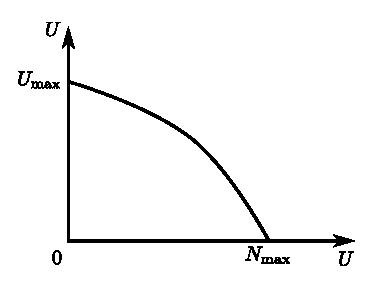
\includegraphics{figures/fig1.1.eps}
\centerline{\bf Fig. 1.1.}
\end{figure}
Rewriting (\ref{eq1.2}) as
$$
N_t + (F(N))_x = 0,
$$
where $F(N) = NU(N)$ is the flux of cars, we see that $F=0$ when $N=0$
and when $N$ is maximum (in this case $U(N)=0$).\pageoriginale Hence
the graph of the flux curve $F(N)$ will look as in figure 1.2. It
could have the shapes as shown in figure 1.2 (a) and 1.2 (b), but
these lead to certain difficulties in the theory. 
\begin{figure}[H]
\centering
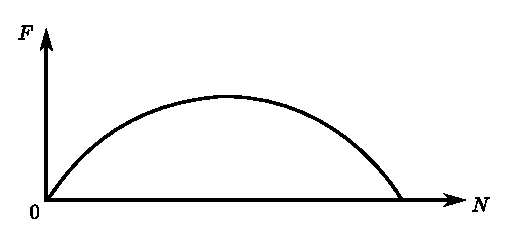
\includegraphics{figures/fig1.2.eps}
\centerline{\bf Fig. 1.2.}
\end{figure}


\noindent
\begin{minipage}[C]{5cm}
\begin{figure}[H]
\centering
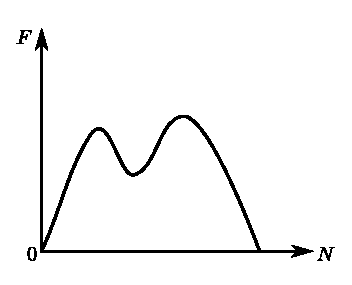
\includegraphics[scale=0.9]{figures/fig1.2a.eps}
\centerline{\bf Fig. 1.2~(a).}
\end{figure}
\end{minipage}
\quad 
\begin{minipage}[C]{5cm}
\begin{figure}[H]
\centering
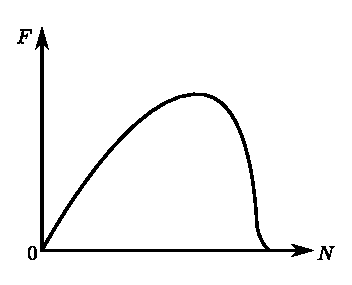
\includegraphics[scale=0.9]{figures/fig1.2b.eps}
\centerline{\bf Fig. 1.2~(b).}
\end{figure}
\end{minipage}

\bigskip

Consider the simplest case in which the flow is steady, i.e., independent of time. Then from (1.3), we obtain
$$
F(N) = \text{ constant}.
$$
In general, the line $F(N) = $ constant, will cut the flux graph in two points as shown in figure (1.3).

\begin{figure}[H]
\centering
\includegraphics{figures/fig1.3.eps}
\centerline{\bf Fig. 1.3.}
\end{figure}

If we\pageoriginale require continuity in $N$, then we have to take either $N = N_1$ or $N = N_2$. If we allow jump discontinuities in $N$, then uniqueness in the solution will be lost as shown in figure (1.4). Then thick line can be a condidate for the solution but the dotted line could also be a candidate for the solution.

So, for uniqueness, we need an additional condition which is called an {\em Entropy Condition}. The terminology will become clear when we study gas dynamics. Again this has to come from the physics of the problem at hand.

For the traffic problem at hand, we would like to add the {\em entropy condition} that infinite acceleration is impossible, i.e.
$$
\frac{\partial U}{\partial x} < \infty (\text{or  }\frac{\partial N}{\partial x} > - \infty). 
$$
It turns out that there is then a unique solution to the initial value problem.

\begin{figure}[H]
\centering
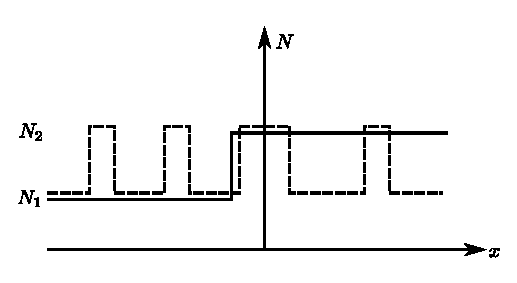
\includegraphics{figures/fig1.4.eps}
\centerline{\bf Fig. 1.4.}
\end{figure}

We also observe that for a given conservation law in differentiated form there are several equivalent conservation\pageoriginale laws in differentiated form. For example, consider 
$$
N_t + (F(N))_x = 0.
$$
Let $P(N)$ be any arbitrary integrable function of $N$. Put 
$$
Q(N) = \int\limits^N_{N_*} P(M) dM.
$$
Then 
\begin{align*}
Q_t & = Q'(N) \cdot N_t\\
& = P(N) \cdot (-\frac{dF}{dN} \cdot N_x)\\
& = -(R(N))_x, \text{ where } R(N) = \int\limits^N_{N_*} P(M) \cdot F' (M) dM.
\end{align*}
Thus
$$
Q_t + R_x =0.
$$

Hence to choose the {\em correct entropy condition, and thus to get
  uni\-queness, we should look at the integrated form of the
  conservation law.} 

If we allow discontinuities in the solution, it is a so-called {\em weak solution}. We shall now give a precise definition of a weak solution for a general first order nonlinear equation and then return to the traffic problem again.

\section{Weak Solutions}\label{chap1:sec1.2}

Consider a first order nonlinear equation
\begin{equation*}
N_t + (F(N))_x = 0, \quad - \infty < x < \infty, \quad t >0. \tag{1.4}\label{eq1.4}
\end{equation*}
Let $N$ be a classical solution of (\ref{eq1.4}). By this we mean that\pageoriginale $N$ is a $C^1$ function in $x,t$ variables and satisfies (\ref{eq1.4}) identically. Let now $\chi(x,t)$ be any $C^\infty$-function (even $C^2$ is enough) which vanishes for large $|x|$ and $t$ and $t =0$.
$$
\int\limits^\infty_{-\infty} \int\limits^\infty_o \chi (x,t) \{N_t + (F(N))_x\} dt \; dx = 0. 
$$
Integrating by parts, we obtain
\begin{equation*}
\int\limits^\infty_{-\infty} \int\limits^\infty_o (\chi_t N + \chi_x F(N)) dt \; dx = 0
\tag{1.5}\label{eq1.5}
\end{equation*}
since the boundary terms vanish. Also, the entropy condition $\dfrac{\partial N}{\partial x} > - \infty$ becomes
$$
\int\limits^\infty_{-\infty} \int\limits^\infty_o \Phi (x,t) \cdot \frac{\partial N}{\partial x} dt \; dx > - \infty
$$
for all $\Phi \geq o$, $C^\infty$ function vanishing for large $|x|$ and $t$ and $t=0$. This again by integrating by parts, becomes 
\begin{equation*}
\int\limits^\infty_{-\infty} \int\limits^\infty_o \Phi_x N \; dt \;  dx < \infty. 
\tag{1.6}\label{eq1.6}
\end{equation*}
Motivated by this, we now define a weak solution.

\begin{defi*}
A locally integrable function $N(x,t)$ is a weak solution of (\ref{eq1.4}) if (\ref{eq1.5}) and (\ref{eq1.6}) hold under the conditions stated there.
\end{defi*}

Note that a classical solution (usually called strong solution) is necessarily a weak solution. Conversely, it can be seen that if $N$ is a weak solution and $N$ is of  class $C^1$ then $N$ is necesaarily a strong solution.

\section{Initial value problem}\label{chap1:sec1.3}
We now consider the problem of solving a general first order nonlinear equation
\begin{equation*}
N_t + (F(N))_x = 0, \quad - \infty < x < \infty, \quad t > 0
\tag{1.7}\label{eq1.7}
\end{equation*}\pageoriginale
with initial data
\begin{equation*}
N(x,0) = \Phi (x), \quad - \infty < x < \infty. \tag{1.8}\label{eq1.8}
\end{equation*}
If we put $G(N) = F'(N)$, (\ref{eq1.7}) can be written as 
\begin{equation*}
N_t + G(N) N_x = 0. \tag{1.9}\label{eq1.9}
\end{equation*}
This we solve by the method of characteristics. If we define a curve $C$ in $x,t$ plane by $dx/dt = G(N)$, we find that on $C$, (\ref{eq1.9}) reduces to 
$$
\frac{dN}{dt} =0,
$$
or $N = $ constant on $dx/dt = G(N) $. Since this means $G(N)$ is also a constant we see that the characteristics are straight lines with slopes $(G(N))^{-1}$. If $x(0) = \xi$ we find that 
$$
N(x,t) = \Phi (\xi) \text{ on } dx/ dt = G(N)
$$
with $x(0) = \xi$. 

Hence we have a solution in implicit form given by 
\begin{equation*}
\left.
\begin{aligned}
& x = \xi + t G (\Phi (\xi)) \quad \\
& N (x,t) = \Phi (\xi)
\end{aligned}
\right\}\tag{1.10}\label{eq1.10}
\end{equation*}
If we can determine $\xi = \xi (x,t)$ from the first equation, then we know $N$ at $(x,t)$ uniquely. But, however, this is not always the case; and trouble occurs if the characteristics intersect, as we shall see now. If $\xi = R$, $\xi = L$ are two points on the $x$-axis such that 
$$
G(\Phi (L)) > G(\Phi (R)) > 0
$$
\begin{figure}[H]
\centering
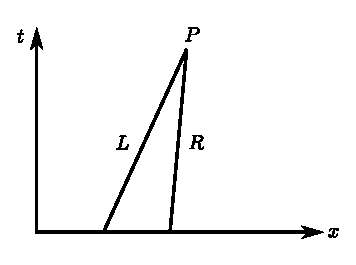
\includegraphics{figures/fig1.5.eps}
\centerline{\bf Fig. 1.5.}
\end{figure}\pageoriginale 
(See figure (1.5)) then the characteristic through $R$ intersects the characteristic through $L$ at $P$. Thus the value of $\xi$ corresponding to the point $P$ is {\em not} unique.

However, if the characteristics fan out, then clearly there will be a unique characteristic through every point and the solution will be determined uniquely. If
\begin{equation*}
G(\Phi (L)) < G (\Phi (R)) \tag{1.11}\label{eq1.11}
\end{equation*}
for $L< R$ then the characteristics in the $x,t$ plane have decreasing slopes and they never intersect. In such  a case, we obtain a unique continuous solution.

Since the solution is given implicitly by (\ref{eq1.10}) another way of looking at the breakdown, when (\ref{eq1.11}) does not hold is to try to solve the first equation in (\ref{eq1.10}) using implicit function theorem. the functional relation
$$
f(x,t, \xi) = 0
$$
can be represented in a single-valued way by
$$
\xi = g(x,t)
$$
if and only if $f_\xi \neq 0$. Put
$$
f(x,t,\xi) = t G (\Phi (\xi)) - (x - \xi).
$$
Then\pageoriginale
$$
f_\xi = t \cdot \frac{dG}{dN} \cdot \frac{d\Phi}{d \xi} + 1.
$$
Hence, if 
$$
\frac{dG}{dN} \cdot \frac{d\Phi}{d\xi}
$$
is always positive for all positive $t$ we have $f_\xi > 0$. On the other hand, if this expression changes sign, there is a finite time, called breaking time, at which $f_\xi = o$. We note from the relations
$$
N_t = - \frac{\Phi' \cdot G(N)}{1+ t \Phi' G'} , \quad N_x \frac{G(N)}{1 + t \Phi' G'} 
$$
that the derivatives in $N$ will blow up at the time of breaking. We also note that the  breakdown in the solution can happen even if the initial data are very smooth. Suppose the flux curve is convex, so that $G' = F'' < 0$. Now, if the initial data $\Phi$ is very smooth and tends to zero as $|x| \to \infty$, then $\Phi'$ will change its sign and there is always a time at which the solution will become singular.

This is true in higher dimensions also. John, F. \cite{key19} has investigated the question of how late with 3-space variables and a nonlinear equation, a breakdown can occur. Note in the above that as $|\Phi'| \to 0$ the breaking time $t \to \infty$. Klainerman \cite{key21} has shown for the nonlinear analogue of the wave equation.
$$
N_{tt} - N + \sum\limits_{i,j} a_{ij} (\nabla N, N_t) \frac{\partial^2 N}{\partial x_1 \partial x_j}  = 0
$$
that if the number of space variables is greater than or equal to 6,\pageoriginale then compact initial data can propagate smoothing for all time. This leaves open the anologous important question in 2 and 3 dimensions.

\begin{exercise}\label{chap1:exer1.1}
Describe the solution of 
$$
N_t + (F(N))_x = 0
$$
with 
\begin{align*}
F(N) & = 16 - N \quad \text{ if } \quad N < 4\\
& = 0 \quad  \text{ if } \quad N > 4
\end{align*}
for the initial data 
\begin{itemize}
\item[{\rm a)}] ~ \qquad  $N (x,0) = 2 - \text{ tanh } x$

\item[{\rm b)}]  
\begin{tabbing}
~ \qquad 
$N (x, 0)$ \= =  \= $2 - \text{ tanh } x $ if $x < 0$\\
\> = \> $2 - \dfrac{1}{2} \text{ tanh } x $ if $x>0$.
\end{tabbing}
\end{itemize}
Where does the discontinuity in $N_x$ move ?
\end{exercise}

\begin{exercise}\label{chap1:exer1.2}
Work out the corresponding theory for 
$$
U_t + a (U) U_x  + b(U) U_y = o
$$
and determine conditions on $a$ and $b$ which lead to discontinuities for all compact initial data.

We now return to our traffic problem and ask how the condition (\ref{eq1.11}) should be interpreted as a condition on the density at some given time.
\end{exercise}

We refer to the flux curve (see figure (1.2)). Suppose $F$ attains a maximum value at density $N_\ast$. Then $F$ is increasing in $[0, N_*]$ and decreasing in $[N_*, N_{\text{Max}}]$. $N_{\text{Max}}$ is the maximum density at which $F=0$. Hence\pageoriginale $G(N) = dF/dN$ is decreasing in $[0, N_*]$, equal to sero at $N_*$ and again decreasing (negatively) beyond $N_*$. Hence the graph of $G(N)$ will look as shown in figure (1.6).

\begin{figure}[H]
\centering
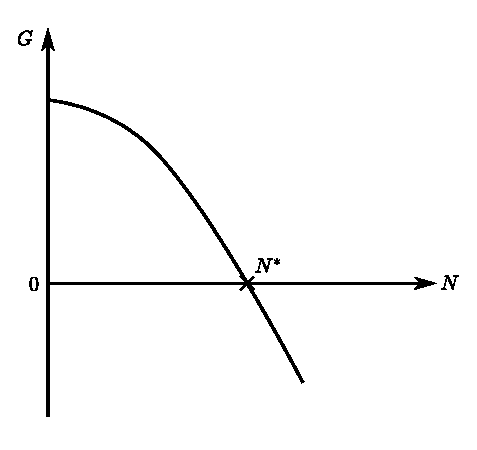
\includegraphics{figures/fig1.6.eps}
\centerline{\bf Fig. 1.6.}
\end{figure}

If the traffic problem is accelerating at the given time, i.e. cars to the right going faster than those to the left then $N$ is a decreasing function of $x$. Thus
$$
N(L) > N(R)
$$
for all pairs $L,R$ such that $L<R$ and thus 
$$
G(N(L)) < G(N(R))
$$
(unless the density has increased beyond $N_*$), so that (\ref{eq1.11}) holds and we have a unique continuous solution. However, the tail of the $G(N)$ curve for $N > N_*$ was fixed up artificially to give us a smooth curve and we should properly speaking ignore this region.

If the traffic is decelerating then $N(L) < N(R)$ for all pairs $L,R$ with $L<R$ and we will not be able to obtain a continuous solution. 

We are\pageoriginale then forced back to re-examine our model. The conservation of the number of vehicles still holds, but we can allow discontinuities in density.

We have the conservation law 
$$
\oint\limits_\epsilon (N dx - Fdt) = 0
$$
for every closed curve $\epsilon$ in the $x,t$ plane or equivalently 
\begin{equation*}
\frac{d}{dt} \int\limits^{x_2}_{x_1} N(x,t) dx + [F(N)]^{x_2}_{x_1} =0 
\tag{1.12}\label{eq1.12}
\end{equation*}
for every segment $[x_1 , x_2]$ if $N$ has jump discontinuities. We ask for piecewise smooth solutions $N$ and investigate what happens across a discontinuity in $N$ as in the steady case. Such a discontinuity is called a {\em shock} and the curve on which it lies is the {\em shock curve}.

A discontinuity in $N$ implies, of course, a discontinuity in the speed $U$. These discontinuities represent instant or rather infinite decelerations. In many situations, the presence of a discontinuity represents a pile-up and to say the least, the model breaks  down. However, densities have been defined in an average sense and if the traffic is this enough a sharp deceleration can occur and we can study what happens to it. Ofcourse, the relation of speed to density {\em inside} this narrow region represented by the discontinuity cannot be the old one.

On the other hand, one might also ask, why not allow discontinuities in an accelerating situation ? It is not quite clear that in a traffic situation one should not but again\pageoriginale it involves violating the speed density relation in some narrow region and this time we would lose uniqueness. 

Let $x = s(t)$ be a $C^1$-function representing the shocks curve. We work with the conservation law given by (\ref{eq1.12}). Let $x_1 < s (t) < x_2$ at some time. Then from (\ref{eq1.12}) we obtain
$$
\frac{d}{dt} \int\limits^{s(t)-}_{x_1} Ndx + \int\limits^{x_2}_{s(t) +} Ndx + F(N) (x_2) - F(N) (x_1) = 0.
$$
Differentiating under the integral sign and taking the limits 
\begin{equation*}
\left.
\begin{aligned}
& x_1 \to s(t) - \quad \\
& x_2 \to s(t) + 
\end{aligned}
\right\} 
\end{equation*}
we obtain 
$$
-S (N_R - N_L) + (F_R - F_L) = 0,
$$
where we denote $ds/ dt$ by $S$ and $N_R, N_L$ and $F_R, F_L$ are the corresponding limiting values from right and left respectively. We then have
\begin{equation*}
S = \frac{F_R - F_L}{N_R - N_L}\tag{1.13}\label{eq1.13}
\end{equation*}
$S$ is called {\em shock speed } and $(N_R - N_L)$ {\em shock strength}. The equation (\ref{eq1.13}) is called a {\em jump condition}.

\begin{exercise}\label{chap1:exer1.3}
If $N$ is a piecewise smooth weak solution of $N_t + (F(N))_x = 0$, show that the jump condition holds across the line of discontinuity. Further, show that as the shock strength goes to zero, the shock speed becomes the characteristic speed.
\end{exercise}

We want\pageoriginale to show that by allowing shocks we can solve any initial value problem uniquely and that we can study in particular where the shock travels and how strong it gets. We first look at {\em constant states}.

The simplest problem to solve is the transition from one constant density, say, $N_R$ to another constant density $N_L$. The deceleration requirement is that $N_R > N_L$. The shock speed, by (\ref{eq1.13}), is the slope of the line segment connecting two points on the flux curve; see figure (1.7).

\begin{figure}[H]
\centering
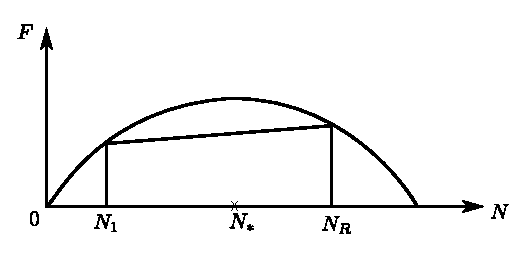
\includegraphics{figures/fig1.7.eps}
\centerline{\bf Fig. 1.7.}
\end{figure}

It is positive or negative depending on the relationship of $N_L$ and $N_R$ to $N_*$. A more important question is whether it is more or less than the speed of the traffic.

Generally speaking, relative to the traffic ahead at time $t$, the shock is always retreating, i.e., $S < U_R$. For, since $F = NU$.
\begin{align*}
S - U_R & = \frac{F_R - F_L}{N_R - N_L} - U_R\\
& = \frac{N_L(U_R - U_L)}{N_R - N_L} < 0, \text{ since } N_R > N_L. 
\end{align*}
Similarly,\pageoriginale $S < U_L$. Thus, all traffic ahead of the shock remains ahead but all traffic behind it eventually hits it and decelerates. The path history of cars is illustrated in figure (1.8).

\begin{figure}[H]
\centering
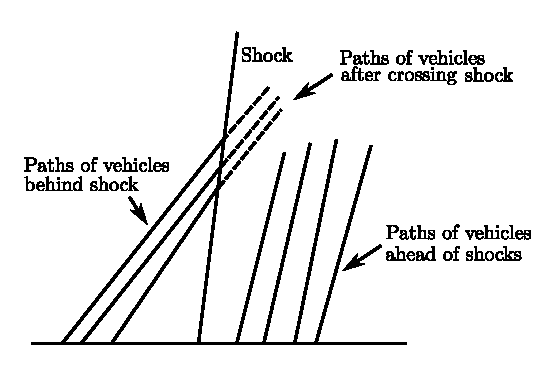
\includegraphics{figures/fig1.8.eps}
\centerline{\bf Fig. 1.8.}
\end{figure}

\section{Initial value problem with shock}\label{chap1:sec1.4}
We already know from the constant configuration (and it can be proved generally) that the vehicles after crossing the shock move off at a slower speed. However, the behaviour of characteristics is quite different; they hit the shock from both sides. In the $x,t$ plane the slope of the characteristic satisfies $dx/dt = G(N) = dF/dN$. From the $G-N$ curve (figure (1.7)), we see that not only $G(N_R) < 0$, but $G(N_R)< S$, for $N > N_*$ since $N_R > N_L$ and $F$ is convex. Hence the characteristics ahead of a shock run into it. Behind the shock the reverse is true, $G(N_L) > S$ and again the characteristics hit the shock (figure (1.9)).

\begin{figure}[H]
\centering
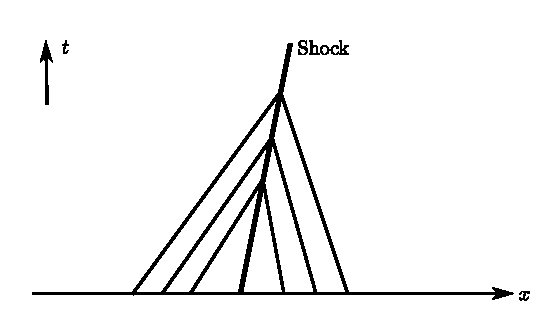
\includegraphics{figures/fig1.9.eps}
\centerline{\bf Fig. 1.9.}
\end{figure}\pageoriginale

If we knew how to {\em lay down} the shock across overlapping characteristics, we could solve the {\em initial value problem}. The shock starts when the continuous method breaks down, i.e., when $\partial N/ \partial x$ becomes infinite at some time and plane. Let this, for the sake of argument, be (0,0). Then initial slope of the shock is the characteristic slope and we integrate from this point (0,0). The shock velocity
\begin{align*}
\frac{dx}{dt} = S & = \frac{F_R - F_L}{N_R - N_L}\\
& = \frac{F(\Phi (\xi_R)) - F (\Phi (\xi_L))}{\Phi (\xi_R) - \Phi (\xi_L)}
\end{align*}
where $\Phi$ is the given initial data and $\xi_R (x,t), \xi_L(x,t)$ are the abscissae of the appropriate right and left characteristics. To find this curve, a useful approximation is often made. We use the subscripts $R$ and $L$ in an obvious manner and note two possibilities of getting Taylor expansions for the shock speed in terms of the shock strength $N_R - N_L$.
\begin{align*}
S = \frac{F_R - F_L}{N_R - N_L} & = (\frac{dF}{dN})_R + \frac{1}{2} (\frac{d^2 F}{dN^2})_R (N_R - N_L) + 0 ((N_R - N_L)^2)\\
& = (\frac{dF}{dN})_L + \frac{1}{2} (\frac{d^2 F}{dN^2})_L (N_L - N_R) + 0  n((N_L - N_R)^2)
\end{align*}\pageoriginale
as $N_R \to N_L$. Adding the two expressions,
\begin{align*}
2S &= \left(\left(\frac{dF}{dN} \right)_R + \left(\frac{dF}{dN}
\right)_L \right) + \frac{1}{2} \left( \left(\frac{d^2 F}{dN^2}
\right)_R - \left(\frac{d^2 F}{dN^2} \right)_L \right)\\
&\qquad\qquad (N_R - N_L) + 0
((N_R - N_L)^2).   
\end{align*}
or, expanding $\left(\dfrac{d^2 F}{dN^2} \right)_R$ and $\left(\dfrac{d^2 F}{dN^2} \right)_L$ in terms of $(N_R - N_L)$, we see that 
$$
S = \frac{1}{2} \left( \left(\frac{dF}{dN} \right)_R + \left(\frac{dF}{dN} \right)_L \right) +  0((N_R - N_L)^2). 
$$
This means the shock speed is the average of the slopes of the two characteristics with a second order error. Note, if $F$ is quadratic the formula is exact.

To find the whole flow in the $(x,t)$-plane, we now have a relatively simple reciple:
\begin{enumerate}
\item Carry $N$ along the characteristics coming from the initial line, i.e., lines of slope $(dF/ dN)^{-1} = G^{-1}$.

\item Note the region where they are crossed.

\item From the points on each line $t =$ constant where such a region starts, start a shock.

\item Integrate the differential equation for the shocks, 
$$
\frac{dx}{dt} = g (x,t),
$$
where $g(x,t) = \dfrac{1}{2} (G_R + G_L)$ is a good approximation.
\end{enumerate}

This procedure is quite straight forward until shocks intersect. But there the initial value problem can be restarted provided we can solve the local problem with 
constant\pageoriginale states on each side. Note if initial data have a discontinuity then the two sides can be connected either by a shock or by a degenerate solution of (\ref{eq1.10}) with $x = t G(N)$ called  a centered wave. However, interaction shows that the number of shocks decreases.

The real numerical difficulty of the foregoing procedure lies in inverting the variable and finding $\xi$ as a function of $x,t$. For this reason, it is often preferable to use a difference scheme. Before going into this, we now give some existence and uniqueness theorems. 

\begin{remarks*}
We note the difference in shock speed if we use different conservation laws that are equivalent in the smooth case. From
$$
N_t + F_x = 0,
$$
we have seen that, $Q$ satisfies
$$
Q_t + T_x =0
$$
where
$$
Q = \int\limits^N P(M) dM
$$
and 
$$
T = \int\limits^N P(M) F'(M) dM. 
$$
Considering shock speeds, we see that 
\begin{align*}
S & = \frac{T_R - T_L}{Q_R - Q_L}\\
& = \frac{\int\limits^{N_R}_{N_L} P(N) F' (N) dN}{\int\limits^{N_R}_{N_L} P(N) dN}
\end{align*}
 In the\pageoriginale limits as $N_L \to N_R$ we see that $S$ tends to the characteristic speed, the same for both the forms. But for $N_R \neq N_L$ we can obtain a wide range of shock speeds by the choice of $P(N)$. 
\end{remarks*}

To get uniqueness, as we shall see, we introduce the following {\em entropy condition} to go with a specific weak conservation law:

{\em The characteristics starting on either side of the discontinuity curve (shock curve) when continued in the direction of increasing time $t$ intersect the line of discontinuity.}

This means the characteristics issuing from a shock go backwards in time (see figure (1.9)). This will be the case if 
$$
F' (N_L) > S > F' (N_R) 
$$
where $N_L$, $N_R$ are the values of $N$ on left and right of the shock curve respectively and $S$ is the shock speed. 

Hereafter, in this section, by a shock, we mean a discontinuity satisfying the jump condition and this entropy condition. For the following results, which we are going to derive, we refer to P.D. Lax \cite{key23}. The most important feature there is the role of the $L^1$ norm. A piecewise continuous function such as a solution with shocks will have its first derivatives in $L^1$ but not in $L^2$. Consider
\begin{equation*}
N_t + F_x = 0, \quad -\infty < x < \infty, \quad t  > 0. 
\tag{1.14}\label{eq1.14}
\end{equation*}
We assume $F$ is convex\footnote{In the traffic problem $F$ is concave but the problem can be transformed to this case.} and a $C^2$-function.

\begin{exercise}\label{chap1:exer1.4}
Let $f: (a,b) \to \mathbb{R}$\pageoriginale be a $C^2$-function. Then $f$ is convex iff $f''(x) > 0$ for all $x \in (a,b)$. Further show that $f$ satisfies the inequality
\begin{equation*}
f(x) \geq f(y) + (x-y) f'(y)\tag{1.15}\label{eq1.15}
\end{equation*}
for all $x,y \in (a,b)$.
\end{exercise}

\begin{theorem*}
Let $N,M$ be two piecewise continuous solutions of (\ref{eq1.14}) whose discontinuities are only shocks. Then $||N-M||(t)$ is a decreasing function of $t$ where
$$
||N-M|| (t) = \int\limits^\infty_{-\infty} |N(x,t) - M (x,t) |dx.
$$
\end{theorem*}

(We assume the integral exists).

\medskip
\begin{coro*}[(Uniqueness Theorem)]
If $N=M$ at time $t = 0$, then $N \equiv M$.
\end{coro*}

\begin{proof}
Let $x = y_n(t)$ be the points such that $(N-M)$ has the sign of $(-1)^n$ in $y_n(t) < x < y_{n+1} (t)$. Then 
$$
|| N - M|| (t) = \sum (-1)^n \int\limits^{y_{n+1}}_{y_n} (N-M) dx.
$$
There are two cases:
\begin{itemize}
\item[{\rm (i)}] Suppose $N = M$ on a curve which is not a shock curve of either solution. Then $G(N) = G(M)$. Thus the two sets of characteristics have the same slopes and hence coincide. Hence there is a segment or a point on every line $t = $ constant where $N = M$. If it is a point, the curve on which $N=M$ is a characteristic; if it is a line segment then the whole region swept out by the characteristics from the segment satisfies $N=M$.

\item[{\rm (ii)}] The curve\pageoriginale where $N=M$ is a shock. Consider 
\begin{align*}
\frac{d}{dt} || N-M|| (t) & = \sum (-1)^n \left\{ \int\limits^{y_{n+1}}_{y_n} (N_t - M_t) dx + \right. \\
& \left. + (N-M) \big|_{y_{n+1}} \frac{dy_{n+1}}{dt} - (N-M) \big|_{y_n} \frac{dy_n}{dt} \right\}.  
\end{align*}
\end{itemize}

Consider the term in the bracket; from equation (\ref{eq1.14}) it is 
\begin{equation*}
\int\limits^{y_{n+1}}_{y_n} (F(M)_x - F(N)_x) dx + (N-M) \frac{dy}{dt}]^{y_{n+1}}_{y_n} \\
= [F(m) - F(N) + (N-M) \frac{dy}{dt}]^{y_{n+1}}_{y_n}, \tag{1.16}\label{eq1.16}
\end{equation*}
where $y_n$ are now points of discontinuity of $N$ or $M$. The contribution from other points $y_n$ vanishes because $N=M$ and $F(M) = F(N)$. Next we calculate the contribution at the upper point $y_{n+1}$. Suppose $N$ has a discontinuity at $y_{n+1}$ and $M$ does not; the other cases are analogous. Now
$$
\frac{dy}{dt} = S = \frac{F(N_L) - F(N_R)}{N_L - N_R}.
$$
Since $(N-M)$ changes sign and $M$ does not have a discontinuity at $y_{n+1}$, we must have 
$$
N_R < M < N_L. 
$$
The contribution of the term in the bracket in (\ref{eq1.16}) at $y_{n+1}$ is thus, with $N=N_L$, given by 
\begin{align*}
& F (M) - F (N_L) + (N_L - M) \cdot \frac{F(N_L) - F(N_R)}{N_L - N_R} = \\
& = F(M) - \left\{ \frac{M-N_R}{N_L - N_R} F (N_L) + \frac{N_L - M}{N_L - N_R} F(N_R)\right\}
\end{align*}\pageoriginale

$\leq 0$, (by the convexity of $F$ since $N_R < M < N_L$). Since $M < N_L$, $(N_L - M)$ is positive and therefore $n$ is even and hence the contribution is negative. Arguing on the same lines, we find similarly that the contribution from the lower point $y_n$ is also negative as well as the contribution when both $N$ and $M$ have shocks. This completes the proof. 
\end{proof}

\begin{remark*}
A similar estimate which yields uniqueness can be made under alternative conditions on $F$, other than convexity.
\end{remark*}

\begin{theorem*}[(A minimum principle)]
Consider the initial value problem
\begin{align*}
& N_t + F_x = 0, \quad -\infty < x < \infty, \quad t > 0, \\
& N(x, 0) = \Phi (x). 
\end{align*}
Let $N(x,t)$ be a continuous and differentiable solution. Let $\Phi \in L'$ (It suffices to assume that $\Phi$ vanishes for large negative $x$). Put
$$
I(x,y, t) = \int\limits^y_{-\infty} \Phi (s) ds + t H (\frac{x-y}{t}),
$$
where 
\begin{equation*}
H(L) = MG (M) - F(M) , \; M = G^{-1} (L), \; G = dF / dM . 
\tag{1.17}\label{eq1.17}
\end{equation*}
Then $N(x,t) = G^{-1} (\dfrac{x-y}{t})$ where $y$ minimizes $I(x,y,t)$.  (Note $G(N) = F'(N)$ is an increasing function of $N$ by our assumption on $F$; so that the inverse $G^{-1}$ exists).
\end{theorem*}

\begin{proof}
Let\pageoriginale
 \begin{equation*}
U (x,t) = \int\limits^{x}_{-\infty} N (y,t) dy,  \tag{1.18}\label{eq1.18}
 \end{equation*}
then 
\begin{equation*}
U_x = N. \tag{1.19}\label{eq1.19}
\end{equation*}
Since $N$ satisfies the differential equation, we obtain
\begin{equation*}
U_t + F (U_x) = 0; \tag{1.20}\label{eq1.20}
\end{equation*}
here we have adjusted the integration constant by putting 
\begin{equation*}
F(0) = 0. \tag{1.21}\label{eq1.21}
\end{equation*}
If (\ref{eq1.15}) is applied with $U_x$ and any number $M$, we obtain 
$$
F(U_x) \geq F (M) + (U_x -M) G(M). 
$$
Or using (\ref{eq1.20}),
\begin{equation*}
U_t + G(M) U_x \leq MG(M) - F(M).\tag{1.22}\label{eq1.22}
\end{equation*}
Let $y$ denote the intercept on the $x$-axis of the line given by $dx/dt = G(M)$ or
\begin{equation*}
(x-y)/t = G(M), \quad t > 0. \tag{1.23}\label{eq1.23}
\end{equation*}
Integrating (\ref{eq1.22}) along this line w.r.t. $t$ from $t=0$, we obtain
\begin{equation*}
U (x,t) - U(y,0) \leq t [MG(M) - F(M)]. \tag{1.24}\label{eq1.24}
\end{equation*}
From (\ref{eq1.23}), we have 
\begin{equation*}
G^{-1} (\frac{x-y}{t}) = M. \tag{1.25}\label{eq1.25}
\end{equation*}
If $H$ is defined by (\ref{eq1.17}), we see that 
\begin{equation*}
U(x,t) \leq U (y,0) + t H (\frac{x-y}{t}) = I (x,y,t). \tag{1.26}\label{eq1.26}
\end{equation*}\pageoriginale
We also note that 
$$
dH/ dL = G^{-1} (L). 
$$
Let $G(0) = c$; then $G^{-1} (c) = 0$. Since $F(0) = 0$, we have $H(c) =0$ and this is its minimum value. The inequality in (\ref{eq1.26}) holds for all choices of $y$. In particular for the value of $y$ for which $M$, given by (\ref{eq1.25}), equals $N(x,t)$, the sign of equality holds in (\ref{eq1.24}) along the whole characteristic $dx/dt = G(N)$ issuing from $(x,t)$. Therefore, the sign of equality holds in (\ref{eq1.26}). This completes the proof.
\end{proof}

\begin{remark}\label{chap1:rem1}
The above theorem holds also for generalised (weak) solutions whose discontinuities are shocks. For, relation (\ref{eq1.20}) is the integral form of the conservation law and so relation (\ref{eq1.26}) is also valid for generalised solutions. Since all discontinuities are shocks every point $(x,t)$ can be connected to a point $y$ on the initial line by a backward characteristic (entropy condition). For this choice of $M$ equality holds in (\ref{eq1.26}). 
\end{remark}

\begin{remark}\label{chap1:rem2}
The converse of the result given in remark \ref{chap1:rem1} is also true. 
\end{remark}

\medskip
\noindent{\textbf{An estimate for large $t$. }} 
In the first theorem, we have found an explicit formula for the solution of an initial value problem in terms of its initial value. Recall
\begin{equation*}
N(x,t) = G^{-1} (\frac{x-y}{t})\tag{1.27}\label{eq1.27}
\end{equation*}
where $y$\pageoriginale minimizes
\begin{equation*}
I (x,y,t) = \int\limits^y_{-\infty} \Phi (s) ds  + t H (\frac{x-y}{t}) . \tag{1.28}\label{eq1.28}
\end{equation*}
We have also seen that $H$ takes its minimum values at  $F(0) = c$ amd $H(c) = 0$. Let 
\begin{equation*}
k = \frac{1}{2} (G^{-1})' (c) = \frac{1}{2} H''(c). \tag{1.29}\label{eq1.29}
\end{equation*}
Assuming $F$ is strictly convex, we have $k > 0$. Suppose there are two positive constants $k_1$, $k_2$ such that 
\begin{equation*}
2k_1 < H'' < 2k_2. \tag{1.30}\label{eq1.30}
\end{equation*}
It follows then from $H(c) = 0$, $H'(0) = 0$ that
$$
H(L) \geq k_1 (L-c)^2. 
$$
Thus
\begin{equation*}
t H (\frac{x-y}{t}) \geq \frac{k_1}{t} (x-y -ct)^2. \tag{1.31}\label{eq1.31}
\end{equation*}
Now we assume $\Phi \in L^1$ and let $||\Phi||$ denotes its $L^1$-norm. Then using (\ref{eq1.28}) and (\ref{eq1.31}), we conclude
\begin{equation*}
- ||\Phi|| + \frac{k_1}{t} (x-y-ct)^2 \leq I (x,y,t). \tag{1.32}\label{eq1.32}
\end{equation*}
But 
$$
I(x,x-ct, t) = \int\limits^{x-ct}_{-\infty} \Phi (s)  ds \leq ||\Phi||
$$
and hence by the minimum principle 
$$
I (x,y,t) \leq ||\Phi ||
$$
at the minimizing function $y$. Combined with (\ref{eq1.31}), we obtain
\begin{equation*}
|\frac{x-y}{t} - c| \leq \left\{ \frac{2||\Phi||}{k_1 t} \right\}^{1/2} = \tilde{m} / \sqrt{t}, \; \text{ say}. \tag{1.33}\label{eq1.33}
\end{equation*}\pageoriginale
From $(G^{-1})' = H'' < 2 k_2$ and $G^{-1} (c) =0$, we have 
$$
|G^{-1} (L)| \leq 2 k_2 |L-c|,
$$
or 
\begin{align*}
|G^{-1} (\frac{x-y}{t}) | & \leq 2 k_2 |\frac{x-y}{t} - c|\\
& \leq 2 k_2 \cdot \tilde{m} / \sqrt{t} = m / \sqrt{t}, \quad \text{say}.
\end{align*}
Thus
$$
|N(x,t)| \leq m/ \sqrt{t}, \text{ \; from (\ref{eq1.27})}.
$$
Now suppose that $\Phi$ vanishes outside $(-A, A)$; then
\begin{align*}
\int\limits^x_{-\infty} \Phi (s) ds  & = 0, \quad \text{if} \quad x , - A\\
& = \text{ constant, if } x> A.
\end{align*}
According to (\ref{eq1.33}), the minimum value of $y$ lies in the interval
$$
x - ct - \tilde{m} \sqrt{t} \leq y \leq x - ct + \tilde{m} \sqrt{t}. 
$$
If $x < ct - \tilde{m} \sqrt{t} - A$, then $y < - A$, where the value of 
$$
\int\limits^y_{-\infty} \Phi (s) ds  
$$
is independent of $y$ and therefore the minimum of $I$ is attained at the point which minimizes $tH(\dfrac{x-y}{t})$; this value is $y = x - ct$. Similarly, if $x > ct + \tilde{m} \sqrt{t} + A$, the minimizing value is $y = x  - ct$. Since $G^{-1} (c) = 0$, we conclude from $N(x,t) = G^{-1} (\frac{x-y}{t})$ that $N(x,t) =0$ for  $x$ outside the interval $(ct - \tilde{m} \sqrt{t} - A , \; ct + \tilde{m} \sqrt{t} + A)$.
This can\pageoriginale be restated as: Every solution $N$ whose initial value vanishes outside a finite interval, at time $t$ vanishes outside on terval whose length is $0 (\sqrt{t})$ and inside this interval it is $0(1/\sqrt{t})$.

In fact, the result can be improved. We state the theorem without proof.

\begin{theorem*}
Define the 2-parameter family of functions $M(p,q)$, $p,q \geq 0$ as
$$
M(x,t; \; p, q) = 
\begin{cases}
(x-ct) / t F''(0) , & \text{ for } ct - \sqrt{pt} < x< ct + \sqrt{qt},\\
0, & \text{ otherwise}
\end{cases}
$$
Let $N(x,t)$ be any solution with shocks of 
$$
N_t + (F(N))_x = 0
$$
where $F$ is convex, $F'(0) = c$. Then
$$
||N - M (p,q)||(t)
$$
tends to zero as $t \to \infty$ where $||\cdot||$ is the $L^1$-norm and 
\begin{align*}
p & = -2 F''(0) \min\limits_y \int\limits^{y}_{-\infty} \Phi (s) ds\\
q & = -2 F''(0) \max\limits_y \int\limits^{\infty}_y \Phi (s) ds.
\end{align*}
\end{theorem*}

\section{Modifications by diffustion and dissipation}\label{chap1:sec1.5}
Consider the first order nonlinear equation
\begin{align*}
& N_t  + NN_x = 0, \; -\infty < x < \infty, \; t >0, \tag{1.34}\label{eq1.34}\\
& \qquad \qquad N(x,0) = \Phi (x), 
\end{align*}
whose solution is implicitly given by 
\begin{align*}
& x = \xi + t \Phi (\xi)\\
& N (x,t) = \Phi (\xi).
\end{align*}\pageoriginale
We have seen that however smooth $\Phi$ may be the solution becomes discontinuous after a finite time, if $\Phi$ has compact support. We want to consider a different model in which we add an extra {\em dissipative term}:
\begin{equation*}
N_t + NN_x = \alpha N_{xx}, \tag{1.35}\label{eq1.35}
\end{equation*}
where $\alpha$ is a small positive number. This is the well-known Burgers' equation that has been utilized by Burgers as a mathematical model of turbulence. By a nonlinear transformation (Cole-Hopf transformation), it is known that (\ref{eq1.35}) can be reduced to the linear heat equation
\begin{equation*}
\Psi_t = \alpha \Psi_{xx}, \tag{1.36}\label{eq1.36}
\end{equation*}
where 
\begin{equation*}
N = -2 \alpha \frac{\Psi_x}{\Psi}.
\end{equation*}
Solving (\ref{eq1.36}) a complete solution of (\ref{eq1.35}) with $N(x,0) = \Phi (x)$ is given by
$$
N(x,t) = \frac{\int\limits^\infty_{\infty} \frac{x-\eta}{t} e^{-\chi/2\alpha} d \eta}{\int\limits^\infty_{-\infty} e^{-\chi/2\alpha} d \eta},
$$
where 
$$
\chi (\eta; x,t) = \int\limits^\eta_o \Phi (\eta') d \eta' + (x-\eta)^2 / 2t
$$
Hence in the case of Burgers' equation a solution exists for all time
ever for discontinuous (bounded, measurable) functions\pageoriginale
$\Phi$. It can be shown, by the method of steepest descent, that as
$\alpha \to 0$ the  solution of the Burgers' equation becomes,
asymptotically, a solution of (\ref{eq1.34}). 

Now instead of putting an extra dissipative term, we put a dispersive term and consider
\begin{equation*}
N_t + N_{xx} = \beta N_{xxx}. \tag{1.37}\label{eq1.37}
\end{equation*}
This is the Kortaweg-deVries equation, originally formulated in the\break
study of shallow water theory. Recently, P.D. Lax and D. Levermore
have developed the theory of the connection between this equation and
shock theory in the limit $\beta \to 0$. Many other mathematical
properties of this equation have been studied in recent years. 

\section{Propagation of singularities in derivatives}\label{chap1:sec1.6}
Let $\Omega = \Omega_1$ $\Omega_2 \Gamma$  be an open set in $(x,t)$ plane (see figure 1.10). Let $f(x,t)$ be a continuous function in $\Omega$. Suppose $f_x$, $f_t$ are continuous in $\Omega_1$ and $\Omega_2$ and have finite limits as they approach $\Gamma$ from either side. Let $\Gamma$ be described by a smooth curve

\begin{figure}[H]
\centering
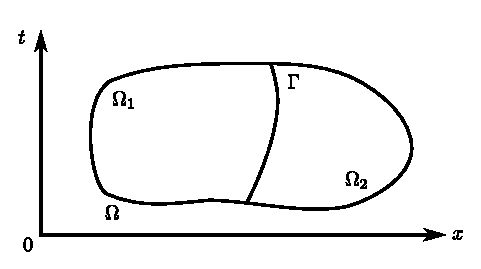
\includegraphics{figures/fig1.10.eps}
\centerline{\bf Fig. 1.10.}
\end{figure}
$x= s (t)$.\pageoriginale Let $[\cdot ]$ denote the jump across $\Gamma$. Then a calculation shows 
\begin{equation*}
\frac{d}{dt} [f] = [f_x] s' + [f_t]. \tag{1.38}\label{eq1.38}
\end{equation*}
Consider now the equation 
\begin{equation*}
N_t + G(N) N_x = 0\tag{1.39}\label{eq1.39}
\end{equation*}
in $\Omega$. Let $N$ be a continuous function in $\Omega$, having discontinuities in $N_x$, $N_t$ across $\Gamma$, and satisfying (\ref{eq1.39}) in $\Omega_1, \Omega_2$. Applying (\ref{eq1.38}) to $N$, we abtain
\begin{equation*}
[N_x] s' + [N_t] = 0, \tag{1.40}\label{eq1.40}
\end{equation*}
since $[N] =0$. 

Since $N$ satisfies (\ref{eq1.39}) in $\Omega_1$ and $\Omega_2$, we obtain as we approach $\Gamma$ that 
\begin{equation*}
[N_t] + G(N) [N_x] = 0. 
\tag{1.41}\label{eq1.41}
\end{equation*}
L\'et $\lambda = [N_x]$; then from (\ref{eq1.40}) $[N_t] = - \lambda s'$. Thus from (\ref{eq1.41}), we obtain 
$$
-\lambda s' + G(N) \lambda = 0.
$$
Assuming $\lambda \neq 0$, we obtain $s' = G(N)$. But then this curve is precisely a characteristic. Hence the discontinuities in $N_x$, $N_t$ propagate along characteristics. 

\begin{note*}
This is true in higher dimensions also. 
\end{note*}

Let us look more closely at the singularities in $N_x$, $N_t$. To do this, we put $p = N_x$, $q = N_t$. Then in the regions where $p,q$ are continuous they satisfy the equations 
\begin{align*}
& p_t + G(N) p_x + G' (N) p^2 = 0, \tag{1.42}\label{eq1.42}\\
& q_t + G(N) q_x + G' (N) pq = 0 \tag{1.43}\label{eq1.43}
\end{align*}\pageoriginale
respectively. Solving (\ref{eq1.42}) by the method of characteristics, we find 
$$
p = \frac{1}{\int\limits^t G'(N)dt - c} \text{ on } dx / dt = G(N),
$$
where $c$ is a constant. Note that the characteristics for these equations and the original equation are the same. Note that since at the time of breaking $p$ becomes infinite, the constant $c$ must become the integral in the denominator at that time. 

\section{Computing methods}\label{chap1:sec1.7}
Although we have obtained a method of solving a nonlinear equation, it may be difficult to obtain the solution  explicitly using the method described. In practice, it is preferable to use a difference scheme.

We first consider a linear equation
$$
U_t + a U_x = 0
$$
where `$a$' is a constant, with initial condition $U(x,0) = \Phi (x)$. Let the domain be approximated by a rectangle. Divide this rectangle into small rectangles of length `$h$' and width `$k$' (see the figure 1.11). We want to find an approximate value of $U$ on this mesh of points. 
\begin{figure}[H]
\centering
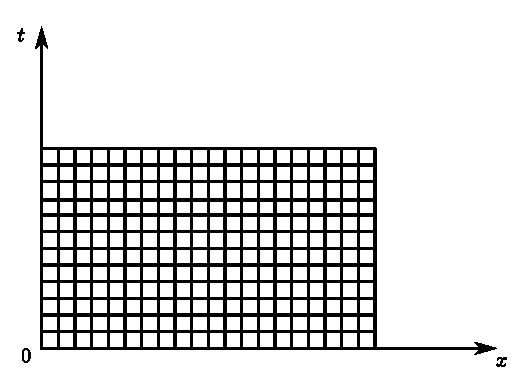
\includegraphics{figures/fig1.11.eps}
\centerline{\bf Fig. 1.11.}
\end{figure}\pageoriginale

Let $U(x,t) = U (hi, kj) = U^j_i$.  The simplest way to approximate $\partial U/\partial t$, at $(hi, kj)$, would be by
$$
\frac{U^{j+1}_i - U^j_i}{k}
$$
making an error of order $k$. We shall this is too inaccurate. If a similar approximation is made for $\partial U/\partial x$ we obtain the following difference equation
$$
\frac{U^{j+1}_i - U^j_i}{k} + a \cdot \frac{U^j_{i+1} - U^j_h}{h} = 0
$$
or 
\begin{equation*}
U^{j+1}_i = U^j_i - \frac{ak}{h} (U^j_{i+1} - U^j_i) \tag{1.44}\label{eq1.44}
\end{equation*}
Its simplicity lies in the fact that it requires the values only on the first row, which will be given by the initial data. Each evaluation, however, gives an error of order $h^2$ or $k^2 = \alpha^2 h^2$, say, and if one substitutes consecutively, the value $U^j_i$ is obtained and involves using the approximation $j(j-1)/2$ times, i.e., making an error of order\pageoriginale $j(j-1)h^2/2$. Now, if $j$ is a mesh corresponding to final time $T$, $j = T/k = T/h$ and, hence, the error behaves like $T^2$. Therefore, we would have to keep $T$ small in order to avoid an error that is of the same size as the solution. In spite of this possibility, the scheme is sometimes useful because of its simplicity. Thus in moving from an ordinary differential equation, we see that we must make a scheme that has more consistent accuracy.

We look now instead for a scheme that is accurate in the equation or {\em consistent with the equation} to second order in the difference $h$ taking $k,h$ of the same order of magnitude.

We note that a derivative is much more accurately described by a difference ratio that straddles equally the point where the approximation is made. Thus using
$$
\frac{U^{j+1}_i - U^{j-1}_i}{2k}
$$
for $\partial U / \partial t$ the derivative is accurate to second order in $k$. This can be seen as follows. Let $W(t)$ possess a Taylor's series. Then
\begin{align*}
W(t + \Delta t) & = W(t) + W' (t) \cdot \Delta t+ W'' (t) \cdot (\Delta t)^2 / 2 + 0 ((\Delta t)^3),\\
W (t- \Delta t) & = W(t) - W' (t) \cdot \Delta t + W'' (t) \cdot (\Delta t)^2 / 2 + 0 ((\Delta t)^3). 
\end{align*}
On subtraction, we obtain
$$
W'(t) = \frac{W(t+ \Delta t) - W(t- \Delta t)}{2\Delta t} + 0 ((\Delta t)^2). 
$$

Thus, we are led to a scheme consistent to $0(h^2)$:
$$
\frac{U^{j+1}_i - U^{j-1}_i}{2k} + a^j_i \frac{U^{j}_{i+1} - U^j_{i-1}}{2h} =0
$$\pageoriginale
or
\begin{equation*}
U^{j+1}_i = U^{j-1}_i - \frac{a^j_i k}{h} (U^j_{i+1} - U^j_{i-1})  
\tag{1.45}\label{eq1.45}
\end{equation*}
Here `$a$' is considered as a function of $x,t$. This algorithm gives us a new row of values from neighbours in the two preceding rows. 

Its apparent disadvantage is that it requires the values on two rows to start with, but we have only one. The simplest way to get the second row is to use the first scheme (\ref{eq1.44}). This leads to an error of order $h^2$ in the second row. This error is just carried through, but not compounded. From the algorithm, we see that the value at the point $(i,j)$ is  obtained successively from a pyramid of mesh points and that the algorithm is applied $j (j-1)/2$ times again; but the error is of order $h^3$ at each step, and hence the error is of order $j^2 h^3$. Since $j \simeq T/ h$, $T$ being the final time, we see that the net error is of order $h$.

This is then a consistent scheme but it is still possible for it to be unstable, i.e., to have the property that it amplifies the error.

\medskip
\noindent{\textbf{Stability. }} (\ref{eq1.45}) (and also (\ref{eq1.44})) is a difference scheme with constant coefficients. A constant raised to a power plays the role that an exponential plays in differential equations. So, we look for solutions of (\ref{eq1.45}) in the form $\xi^i \zeta^j$, i.e.,\pageoriginale $U^j_i = \xi^i \zeta^j$. Substituting this in (\ref{eq1.45}), we obtain a relation between $\xi$ and $\zeta$.
$$
\zeta = \zeta^{-1} - \frac{ak}{h} (\xi - \xi^{-1}). 
$$
Thus for every $\xi$ there are two possible value for $\zeta$. We are, of course, looking for real solutions and we could generate the solutions with real $\zeta$. But, clearly, if $\xi$ and $\zeta$ are complex, then 
$$ 
(\xi^i \zeta^j + {\overline{\xi}}^i {\overline{\zeta}}^j)/2 \quad \text{and} \quad  (\xi^i \zeta^j - {\overline{\xi}}^i {\overline{\zeta}}^j)/ 2 \sqrt{-1},
$$ 
will both be real solutions. For $j=0$, these solutions are $|\xi|^i \cos (i \arg  \xi)$, $|\xi|^i \sin (i \arg \xi)$. If we take $|\xi| =1$ and put $\arg \xi / h = n$, $n=0$, $\pm 1$, $\pm 2, \ldots $ the corresponding values for $j=0$ then become $\cos (nih)$ and $\sin(nih)$, which can be used to describe any initial data by a Fourier series approximation. Let us consider first $\cos(nih)$. At an arbitrary row $j$ its value, since $|\xi| = 1$, is $\re [\exp (\sqrt{-1} \; inh) \zeta^j]$  where we can take $\zeta$ to be either root of 
\begin{align*}
\zeta & = \zeta^{-1} - \frac{ak}{h} (e^{\sqrt{-1}.nh} - e^{-\sqrt{-1}.nh})\\
& = \zeta^{-1} - \frac{2ak}{h} \sqrt{-1} \cdot \sin (nh). 
\tag{1.46}\label{eq1.46}
\end{align*}
Note that the absolute value of the product of the roots is 1. So, if one of the roots has absolute value different from 1, then there is a root with absolute value greater than 1. Suppose $j = T/k$; then the solution is 
$$
|\zeta|^{T/k} \re [e^{\sqrt{-1}(\inh)} \cdot e^{\sqrt{-1}\cdot T /k \cdot \arg \zeta} ]. 
$$\pageoriginale
If the mesh size $k$ shrinks, this solution behaves like $\exp ((T \log \zeta)/k)$ and it also oscillates. The exponential factor goes to infinity as $T$ tends to infinity. A small multiple of this solution even, say, of order $k^3$, for the sake of argument, still goes to infinity. Such a small multiple can easily represent an error and hence, the error amplifies as the mesh size shrinks, i.e., the scheme is unstable unless $|\zeta| = 1$. In that case set $\zeta = \exp (\sqrt{-1} \Phi)$, with $\Phi$ a real. From (\ref{eq1.46}), we then obtain
$$
2 \sqrt{-1} \sin\Phi = - 2 \sqrt{-1} \frac{ak}{h} \sin(nh)
$$
or
$$
\sin \Phi = - \frac{ak}{h} \sin (nh). 
$$
But this has a solution iff $|\dfrac{ak}{h}| \leq 1$, and hence if this is the case the difference scheme is stable. If $|\dfrac{ak}{h}| > 1$, then there is a root $\zeta$ with $|\zeta| > 1$ and the difference scheme is unstable.

What has been established here is the Courant-Friedrichs-Lewy condition for the particularly simple hyperbolic system of one equation.

\begin{note*}
If we look at the characteristics, we see that $h/k$ must be greater than characteristic speed for stability. Otherwise, we are trying to evaluate a solution at points whose domains of dependence include points from which we are drawing no data. 
\end{note*}

\begin{exercise}\label{chap1:exer1.5}
Find the\pageoriginale stability criterion for (\ref{eq1.44}). 

We now consider a difference scheme for the nonlinear equation\footnote{The nonlinear system can be handled inthe same way both formally and numerically proviced the speeds of propagation are always distinct.}
\begin{equation*}
U_t + F_x = 0, \quad - \infty < x < \infty, \quad t>0. 
\tag{1.47}\label{eq1.47}
\end{equation*}
Here $U$ is a scalar and $F(U)$ is smooth. Initial data will be prescribed for (\ref{eq1.47}):
\begin{equation*}
U(x,0) = \Phi (x). \tag{1.48}\label{eq1.48}
\end{equation*}
We know that in general smooth solutions of (\ref{eq1.47}) do not exist for all time however smooth $\Phi$ may be; we have to consider weak solutions. We recall the definition:
\end{exercise}

\begin{defi*}
A locally integrable function $U(x,t)$ is a weak solution of (\ref{eq1.47}) with initial data (\ref{eq1.48}) if 
\begin{equation*}
\iint\limits_{t > 0} (W_t U + W_x F) dx dt + \int W (x,0) \Phi (x) dx = 0
\tag{1.49}\label{eq1.49}
\end{equation*}
is satisfied for all smooth functions $W$ which vanish for large $|x|, t$ and $t=0$; we call such functions, test functions. 

We now propose and discuss a difference scheme for getting an approximate solution to (\ref{eq1.47}) with initial data (\ref{eq1.48}).

Choose $G:\mathbb{R}^{2\ell} \to \mathbb{R}$, smooth enough, related to $F$ by the reouirement
\begin{align*}
& \underbrace{G(u, \ldots, u)}_{2\ell - \text{ arguments.}} = F (u). 
\tag{1.50}\label{eq1.50}\\
\end{align*}
For $k$ an integer put $U_k = U (x+ k \Delta x, t)$ where $\Delta x$ is step size in $x$-direction; similarly, let $\Delta t$ be step size in\pageoriginale $t$-direction. Define
$$
G(x + \frac{1}{2} \Delta x)= G(U_{-\ell + 1}, U_{-\ell + 2, \ldots , } U_\ell)
$$
and
$$
G(x-\frac{1}{2} \Delta x) = G(U_{-\ell}, U_{-\ell + 1}, \ldots , U_{\ell -1}). 
$$
We now consider the following difference analog of (\ref{eq1.47})
\begin{equation*}
\frac{\Delta U}{\Delta t} + \frac{\Delta G}{\Delta x} = 0
\tag{1.51}\label{eq1.51}
\end{equation*}
where 
\begin{align*}
\Delta U & = U (x, t + \Delta t) - U (x,t),\\
\Delta G & = G (x + \frac{1}{2} \Delta x) - G(x - \frac{1}{2}\Delta x). 
\end{align*}
It follows from (\ref{eq1.51}) that 
\begin{equation*}
U(x,t + \Delta t) = U (x,t) - \lambda \Delta G, 
\tag*{$(1.51)'$}\label{eq1.51'}
\end{equation*}
where $\lambda = \Delta t / \Delta x$.

We claim that the difference scheme (\ref{eq1.51}), as a consequence of (\ref{eq1.50}), is `consistent' with the differential equation (\ref{eq1.47}) in the following sense: denote by $V(x,t)$ the solution of the difference scheme where, we have taken $V(x,0) = \Phi (x)$. Here $V$ is defined for non-integer multiples $t$ of $\Delta t$, for the sake of convenience, as equal to $V(x,t')$, $t' = [t /\Delta t ] \Delta t$. Ofcourse, $V$ depends on $\Delta x$, $\Delta t$. 

Then the following theorem holds.
\end{defi*}

\begin{theorem*}
Assume that as $\Delta x$, $\Delta t \to 0$, $V(x,t) \to U(x,t)$ boundedly a.e. Then $U(x,t)$ is a weak solution of (\ref{eq1.47}) with initial data (\ref{eq1.48}).
\end{theorem*}

\begin{proof}
Multiply\pageoriginale (\ref{eq1.51}) throughout by $\Delta t$ and by any test function $W$ and then integrate with respect to $x$ to obtain
$$
\int W(x,t) \frac{\Delta V}{\Delta t} dx \; \Delta t + \int W(x,t) \frac{\Delta G}{\Delta x} dx \; \Delta t = 0. 
$$
Now sum over all $t$ which are integral multiples of $\Delta t$ and carry out summation by parts in the first integral; we obtain
\begin{align*}
& \sum\limits_{t >0} \int \frac{W(x,t - \Delta t) - W(x,t)}{\Delta t} V (x,t) dx \; \Delta t - \int W (x,0) \Phi (x) dx + \\
& \qquad \qquad  + \sum\limits_t \int  W (x,t) \frac{\Delta G}{\Delta x} dx \; \Delta t = 0.
\end{align*}
In the last integral replace $x$ by $x- \dfrac{1}{2} \Delta x$ in first term and by $x + \dfrac{1}{2} \Delta x$ in second term; we finally obtain 
\begin{align*}
& \sum\limits_{t>0} \int \frac{W(x,t - \Delta t) - W(x,t)}{\Delta t} V(x,t) dx \; \Delta t - \\
& \qquad \qquad - \int  W (x,0) \Phi  (x) dx\\
&\qquad\qquad - \sum\limits_t \int \frac{W(x+1/2 \; \Delta x) - W(x - 1/2 \; \Delta x) }{\Delta x} G d x \Delta t, 
\end{align*}
where $G$ stands for $G(V_1, \ldots , V_{2\ell})$, $V_1, \ldots, V_{2\ell}$ denoting values of $V$ at $2\ell$ points which are distributed symmetrically around $(x,t)$ and have distance $\Delta x$ from each other. If $V \to U$ boundedly a.e. as $\Delta x$, $\Delta t \to 0$ so do $V_1, \ldots, V_{2\ell}$ and therefore
$$
G(V_1, \ldots , V_{2\ell}) \to G(U, \ldots , U) = F(U) \quad \text{ by (\ref{eq1.50}).}
$$
The proof is complete.
\end{proof}

The real difficulty is to find when $V(x,t) \to U (x,t)$ boundedly.

We turn\pageoriginale to the problem of choosing $G$ and minimizing the truncation error. Let $U(x,t)$ be an exact smooth ($C^2$ is enough) solution of (\ref{eq1.47}). It will then satisfy difference equation \ref{eq1.51'} only approximately; the deviation of right side from the left side of \ref{eq1.51'} is called truncation error. It is easily seen that, in view of (\ref{eq1.50}), then truncation error is $0(\Delta t^2)$. We shall now show, by taking $\ell =1$, that $G$ can be so chosen that the truncation error is $0(\Delta t^3)$. Let
\begin{equation*}
U(x,t + \Delta t) = U (x,t) + \Delta t \; U_t + \frac{1}{2} (\Delta t)^2 U_{tt} + 0 (\Delta t^3)\tag{1.52}\label{eq1.52}
\end{equation*}
be a Taylor series up to terms of second order.

From (\ref{eq1.47}), we obtain the  following:
\begin{equation*}
\begin{split}
& U_t + F_x = 0 \\
& U_{tt} + (A^2 U_x)_x = 0. 
\end{split}\tag{1.53}\label{eq1.53}
\end{equation*}
The second of these equations follows from the calculation with\break $dF/dU = A$,
$$
U_{tt} = -F_{xt} = - F_{tx} = -(AU_t)_x = -(AF_x)_x = -(A^2 U_x)_x.
$$
What is significant is that all $t$ derivatives are exact $x$
derivatives and therefore can be approximated by exact $x$
differences. Substituting\break (\ref{eq1.53}) in (\ref{eq1.52}), we obtain 
\begin{equation*}
U(x,t + \Delta t) = U(x,t) + (\Delta t F + \frac{1}{2} (\Delta t)^2 A^2 U_x)_x + 0 (\Delta t^3). \tag*{$(1.52)'$} \label{eq1.52'}
\end{equation*}
Comparing \ref{eq1.51'} and \ref{eq1.52'}, we see that the truncation error is $0(\Delta t^3)$, iff 
$$
\frac{\Delta G}{\Delta x} = (F + \frac{1}{2} \Delta t \; A^2 U_x)_x + 0 (\Delta t^2). 
$$\pageoriginale
From this, we can easily determine the form that $G$ must take.

\begin{theorem*}
The truncation error in the difference scheme \ref{eq1.51'} is $0(\Delta t^3)$ iff
\begin{equation*}
G(a,b) = \frac{F(a) + F(b)}{2} + \frac{1}{2} \lambda A^2 \cdot (b-a) \tag{1.54}\label{eq1.54}
\end{equation*}
plus terms which are $0(|a-b|^2)$ for $(a-b)$ small.
\end{theorem*}

The quantity $A^2$ in (\ref{eq1.54}) shall be taken as $1/2 \{A^2 (a) + A^2 (b)\}$ for the sake of symmetry more than anything else; any other choice would make a difference that is quadratic in $(a-b)$.

Denote the function in (\ref{eq1.54}) by $G_o$; any permissible $G$ can then be written in the form 
\begin{equation*}
G = G_o + \frac{1}{2} Q (a,b) \cdot (b-a)\tag{1.55}\label{eq1.55}
\end{equation*}
where $Q(a,b)$ vanishes for $a=b$. Substituting (\ref{eq1.55}) in \ref{eq1.51'}, we see that
\begin{equation*}
U(x,t + \Delta t) = U (x,t) + \lambda \Delta' F + \frac{1}{2} \lambda^2 \Delta A^2 \Delta U + \frac{1}{2} \lambda \Delta Q \Delta U, \tag{1.56}\label{eq1.56}
\end{equation*}
where $\Delta' = 1/2 [T (\Delta x) - T (-\Delta x)]$ and $\Delta = T (\dfrac{1}{2} \Delta x) - T (-\dfrac{1}{2} \Delta x)$, $T(s)$ being the shift operator of the independent variable by an amount $s$. We shall call $Q$ the {\em artificial viscosity}.

The difference equation (\ref{eq1.56}) expresses the value of $U$ at time $t + \Delta t$ as a nonlinear function of $U$ at time $t$; we shall write this as
\begin{equation*}
U(t + \Delta t) = N U(t).
\tag*{$(1.56)'$}\label{eq1.56'}
\end{equation*}
The value\pageoriginale of the solution of the difference equation at some later time $k\Delta t$ is obtained from the initial values by the application $k$-times power of the operator $N$.

Our aim is to show that the difference scheme (\ref{eq1.56}) is convergent if the size of $\lambda$ is suitably restricted. In the case of linear equations, it is well-known and easy to show that convergence is equivalent to stability defined as the uniform boundedness of all powers $N^k$ of $N$ with some fixed range $k\Delta t \leq T$, a problem which we have studied previously. In the nonlinear case, following Von Neumann the convergence of the scheme would depend on the stability of the {\em first variation} of the operator $N$. The first variation of $N$, by definition, is a linear difference operator with variable coefficients; Von Neumann has conjectured that such an operator is stable iff all the {\em localized} operators associated with it, i.e., the operators obtained by replacing the variable coefficients by their value at some given point, are stable. 

\medskip
{\textbf{We content ourselves with: }}

\begin{theorem*}
If the Courant-Friedrichs-Lewy condition
\begin{equation*} 
\frac{\Delta x}{\Delta t} \geq |A|_{\rm max} \tag{1.57}\label{eq1.57}
\end{equation*}
is satisfied, the difference equation (\ref{eq1.56}) satisfies Von Newmann's condition of stability that the linearized equation is stable.
\end{theorem*}

\begin{proof}
The first variation of the operator $N$ can be easily computed and is given by 
\begin{equation*}
I + \lambda A\Delta' + \frac{1}{2} \lambda^2 A^2 \Delta^2 + 0 (\Delta x), 
\tag{1.58}\label{eq1.58}
\end{equation*}\pageoriginale
where $\Delta',\Delta$ are as before, and $0 (\Delta x)$ denotes an operator bounded in norm by $|\Delta x |$, provided we are perturbing in the neighbourhood of a smoothly varying solution, i.e., one where neighbouring values differ by $0(\Delta x)$. In this case, the influence of the additional viscosity term is $0(\Delta x)$; see Remark \ref{chap1:rem1} below. 

To {\em localise} the operator (\ref{eq1.58}), we replace $A$ by its value at some point. After making a Fourier transform, the operator $\Delta'$ becomes multiplication by $i \sin \alpha$, and the operator $\Delta$ multiplication by $2i \sin (1/2) \alpha$, so that $(1/2)\Delta^2$ becomes multiplication by $\cos \alpha -1$; here $\alpha = \xi \Delta x$, $\xi$ being dual variable. Hence the amplification function of the operator (\ref{eq1.58}) is 
\begin{equation*}
I + i \lambda A \sin \alpha + \lambda^2 A^2 (\cos \alpha -1) + 0 (\Delta x). 
\tag{1.59}\label{eq1.59}
\end{equation*}
Since the eigenvalues $k$ of $A$ are real, the eigenvalues $v$ of the matrix (\ref{eq1.59}) are given by 
\begin{align*}
|v|^2 & = (1-k^2 (1-\cos \alpha))^2 + k^2 \sin^2 \alpha + 0 (\Delta x)\\
& = 1 - 2k^2 (1-\cos \alpha) + k^4 (1-\cos \alpha)^2 + k^2 (1-\cos^2 \alpha) + 0 (\Delta x)\\
& = 1 - (k^2 - k^4) (1- \cos \alpha)^2 + 0 (\Delta x). 
\end{align*}
By our assumption (\ref{eq1.57}) $|k| \leq 1$. Thus $|v| \leq 1+ 0(\Delta x)$. 

The proof of completed.
\end{proof}

\setcounter{remark}{0}
\begin{remark}\label{chap1:rem1+}
We have seen above that the quadratic terms, $Q(a,b)$, appearing in a representation of $G(a,b)$ influence neither the order of the truncation error nor the stability of the scheme at points where the solution varies smoothly.\pageoriginale The terms do influence, however, at the points where solution varies rapidly, e.g., across a shock. For a detailed analysis, we refer to Lax and Wendroff \cite{key24}.
\end{remark}

As a second example, we consider the Lax-Friedrichs scheme for (\ref{eq1.47}). We add a dissipative term $\epsilon U_{xx}$ with $\epsilon = 2\Delta x^2 / \Delta t$. This scheme is given by 
\begin{equation*}
U^{n+1}_j = U^n_j - \frac{\Delta t}{2 \Delta x} [F(U^n_{j+1}) - F (U^n_{j-1})] + \frac{1}{2} (U^n_{j+1} + U^n_{j} - 2U^n_j),  \tag{1.60}\label{eq1.60}
\end{equation*}
where $U^n_j$ abbrevates $U(j\Delta x, n \Delta t)$. We want to establish convergence via the contraction mapping principle. We write (\ref{eq1.60}) as 
\begin{equation*}
U^{n+1} = T(U^n). \tag*{$(1.60)'$}\label{eq1.60'}
\end{equation*}
Then $T$ maps sequence $\left\{U_j \right\}^\infty_{j = - \infty}$ to a sequence $\Big\{T (U) \Big\}^\infty_{j = - \infty}$ according to 
$$
\{T(U)\}_j = U_j - \frac{\Delta t}{2 \Delta t} [F(U_{j+1}) - F(U_{j-1})] + \frac{1}{2} (U_{j+1} + U_{j-1} - 2U_j). 
$$
Let $\ell^1$ be the space of all summable sequences $\left\{U_j \right\}^\infty_{j=-\infty}$ with usual ordering: if $U, V \in \ell^1$ say $U \leq V$ if $U_j \leq V_j$ for all $j$. Let $a < 0 < b$ and put
$$
C = \{U \in \ell^1 : a < U_j <b \text{ for all } j\}.  
$$
Assuming $F(U_j) - F(U_{-j}) \to 0 $ as $j \to \infty$ it can be seen easily that 
$$
\sum\limits^\infty_{j=-\infty} \{T(U)\}_j = \sum\limits^\infty_{j=-\infty} U_j.  
$$
Thus $T$\pageoriginale is {\em integral preserving}. It is also easy to see that if $\Delta t/\Delta x |F' (\Omega)| < 1$, $a \leq \Omega \leq b$, then $T$ is order preserving, i.e., $U \leq V$.

$T (U) \leq T(V)$. Then it follows, by the following theorem, that $T$ is also a contraction. Thus the scheme is convergent.

\begin{theorem*}
Let $\Omega$ be a measurable space with a positive  measure and $T: L^1 (\Omega) \to L^1(\Omega)$ satisfy
$$
\int\limits_\Omega Tf = \int\limits_\Omega f.
$$
Let $C$ $L'(\Omega)$ be such that whenever $f$, $g \epsilon C$, $\max (f,g) \in C$. Then the following statement are equivalent.
\begin{itemize}
\item[{\rm i)}] $f$, $g\in C$, $f \leq g$ a.e. $T(f) \leq T(g)$: order preserving. 

\item[{\rm ii)}] $\int\limits_\Omega (Tf - Tg)^+ \leq \int\limits_\Omega (f-g)^+$, $f$, $g \in C$ where $r^+ = \max (r,0)$.

\item[{\rm iii)}] $\int\limits_\Omega |Tf - Tg| \leq \int\limits_{\Omega} |f-g|$, $f$, $g \in C$: contraction.
\end{itemize}
\end{theorem*}

For proof, we refer to Crandall and Tartar \cite{key7}.
